
\section*{Exercice 1 - Le marchand de sable}
On se propose de modéliser la constitution d'un tas de sable ainsi que l'écoulement des grains dans un sablier. Afin de simplifier le problème, on se restreindra à travailler en 2 dimensions. Le tas sera modélisé par une pile de grains de sable. 


Dans le cas du sablier, les grains tombent toujours sur la même pile. Le processus de constitution de la pile est le suivant : 
\begin{center}
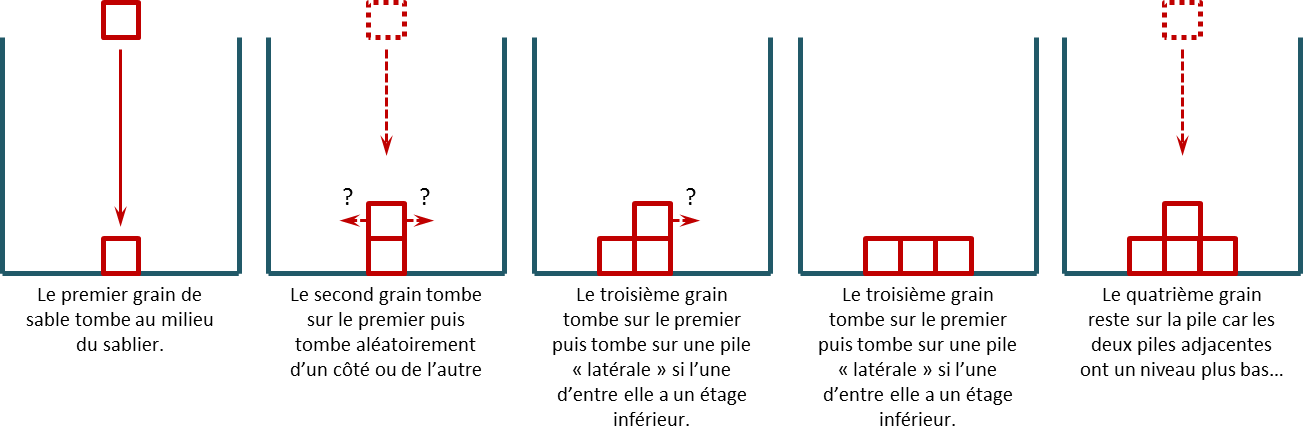
\includegraphics[width=\linewidth]{images/sablier_02}
\end{center}
%Un algorithme très succinct présente le déroulement de la chute d'un grain de sable.
%\begin{center}
%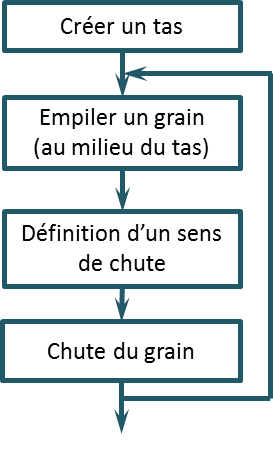
\includegraphics[width=.4\linewidth]{images/algo}
%\end{center}
\subsection*{Gestion d'une pile de sable}

\begin{obj}
Modéliser l'écoulement d'un grain de sable sur une colonne. 
\end{obj}


Une pile de sable est modélisée par... une pile ! Cette dernière est implémentée sous forme d'une liste. 
La taille des piles est de dimension finie notée $\texttt{ht}$. 
Une pile de 3 grains de sable dans une pile de taille 5 sera modélisée par la liste \texttt{['*','*','*','','']}.


\subparagraph{}
\textit{Donner l'implémentation des fonctions élémentaires permettant de gérer une pile dans Python à savoir les fonctions \texttt{creer\_pile}, \texttt{empiler}, \texttt{depiler}, \texttt{est\_vide}. \textbf{Pour cette question on s'autorise l'utilisation des méthodes sur les listes.} \textbf{Vérifier le bon comportement de vos fonctions.}}


\subparagraph{}
\textit{Donner l'implémentation de la fonction \texttt{taille\_pile}, permettant de connaître la taille d'une pile. \textbf{Pour cette question seules les fonctions définies ci-dessus sont acceptées.} Donner la complexité algorithmique de la fonction implémentée. \textbf{Vérifier le bon comportement de vos fonctions.}}

\subparagraph{}
\textit{Implémenter une fonction \\ \texttt{simulation\_pile} prenant comme arguments la hauteur de la pile et le nombre de grains à faire tomber. Cette fonction devra retourner une liste de piles de grain de sables. Cette liste stockera donc les différents états de la pile au fur et à mesure de la chute des grains.}


\subparagraph{}
\textit{Utiliser la fonction  \texttt{trace\_ecoulement} pour tracer l'écoulement des grains sur une pile.}




\subparagraph{}
\textit{Redéfinir la fonction \texttt{empiler} en la nommant \texttt{empilerSable} pour que le seul élément empilable soit la chaîne de caractères "*". Ainsi, une pile de sable sera constituée d'une pile d'étoiles. }

\subsection*{Gestion du tas de sable}
\begin{obj}
L'objectif est de modéliser les fonctions élémentaires afin de pouvoir manipuler un tas de sable et pas une colonne de sable.
\end{obj}

Un tas de sable est maintenant modélisé par une \textbf{liste de piles} de grains de sable appelée \texttt{sablier}. 

\subparagraph{}\textit{Implémenter la fonction \\ \texttt{creation\_sablier} d'arguments \texttt{larg} et \texttt{haut} permettant de créer un sablier constitué de \texttt{larg} piles de hauteur \texttt{haut}.}


\subparagraph{}\textit{Modifier les fonctions \texttt{empiler} et \texttt{depiler} de telles sortes qu'elles prennent comme argument un \texttt{sablier} et un numéro de colonne \texttt{col}. On pourra ainsi déposer ou supprimer un grain de sable sur une colonne \texttt{col} .}

\subsection*{Modélisation de la chute libre d'un grain}

\begin{obj}
On souhaite commencer par simuler la chute libre d'un seul grain.
\end{obj}

Pour observer la chute d'un grain, on stockera dans une variable \texttt{simu} les différents états de la variable \texttt{sablier}. Ainsi \texttt{simu} est une liste de \texttt{sablier}.

\subparagraph{}\textit{Implémenter la fonction \\ \texttt{chute\_libre\_grain} d'arguments \texttt{sablier}, \texttt{col} (numéro de la colonne ou le grain chute) et \texttt{simu}. Cette fonction retourne la variable \texttt{simu}. }


\subparagraph{}\textit{Visualiser la chute d'un grain en utilisant la fonction \texttt{trace\_sablier} . }

\subsection*{Modélisation de la chute d'un grain}
\begin{obj}
Dans un premier temps pn considère que le grain tombe toujours d'un même côté (à gauche par exemple). 

On souhaite simuler ce comportement. 
\end{obj}


Le comportement attendu est le suivant : 
\begin{itemize}
\item le premier grain tombe et reste dans la même colonne;
\item le second grain tombe dans la même colonne puis tombe dans la colonne de gauche;
\item le troisième grain tombe dans. Il ne peux pas tomber à gauche puisque la place est prise. Il reste au même endroit;
\item le quatrième grain tombe dans la première colonne, puis tombe dans la colonne immédiatement à gauche, puis tombe une seconde fois;
\item ...
\end{itemize}


\subparagraph{}\textit{Implémenter la fonction \\ \texttt{chute\_grain} d'arguments \texttt{sablier}, \texttt{col} et \texttt{simu}. Cette fonction retourne la variable \texttt{simu}. }


\subparagraph{}\textit{Implémenter la fonction \\ \texttt{simulation} d'arguments \texttt{nbgrains}, \texttt{larg} et \texttt{haut}. Cette fonction permet de déterminer tous les états du sablier permettant de simuler la chute de \texttt{nbgrains} dans un sablier de largeur \texttt{larg} et de hauteur \texttt{haut}. Cette fonction retourne la variable \texttt{simu}. }

\subparagraph{}\textit{Visualiser la chute de 10 grains en utilisant la fonction \texttt{trace\_sablier} . }


\subsection*{Synthèse}


On identifie les 3 cas suivants pour déterminer le sens de chute d'un grain :
\begin{center}
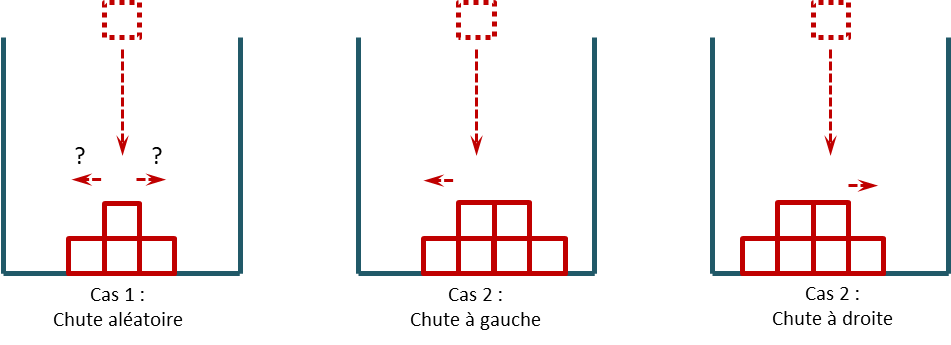
\includegraphics[width=\linewidth]{images/sablier_03}
\end{center}

\subparagraph{}\textit{Simuler et visualiser la chute de 10 grains après avoir modifié la fonction \texttt{chute\_grain} pour que les grains puissent chuter à gauche ou à droite . }


%
%\subparagraph{}\textit{Donner les instructions permettant de dépiler un grain de sable sur la pile $i$ et d'empiler un grain de sable sur la pile $i-1$ du tas à n piles. Tester les instructions pour la pile $i=2$ du \texttt{tasSable=[[],["*"],["*","*","*"],["*"],["*","*"]]}.}
%\section*{Écoulement}
%On va maintenant implémenter les fonctions qui vont permettre de régir l'écoulement d'un grain de sable. On suppose que les grains tombent toujours sur la même pile. 
%
%On s'intéresse d'abord au sens d'écoulement d'un grain de sable. Pour cela, on définit une variable \texttt{sens} qui vaut 0 lorsque le grain doit s'écouler vers la gauche et qui vaut 1 lorsque le grain doit s'écouler vers la droite.
%
%\textbf{On compare la taille des piles avant que le grain de sable soit tombé.
%}
%\subparagraph{}
%\textit{Exprimer la condition booléenne pour laquelle un grain de sable chute à gauche.}
%
%\subparagraph{}
%\textit{Exprimer la condition booléenne pour laquelle un grain de sable chute aléatoirement à gauche ou à droite.}
%
%\subparagraph{}
%\textit{En réalisant un schéma, donner un cas de figure pour lequel il n'y a pas d'écoulement de grain. Traduire la condition booléenne correspondante.}
%
%\subparagraph{}
%\textit{Exprimer la condition booléenne permettant de savoir si un grain qui tomberait sur la pile $n$ doit s'écouler sur la gauche. On tiendra compte du cas où le grain est sur le bord du sablier. }
%
%\subparagraph{}
%\textit{Implémenter la fonction \texttt{sens} permettant de déterminer le sens de la chute du grain : droite, gauche ou si le grain tombe sur sa pile. Cette fonction prendra comme arguments tas(liste de piles) et indice(int) l'indice de la pile sur laquelle le grain sera laché.}
%
%\vspace{.25cm}
%
%On appelle \texttt{chute} la fonction permettant de régir la chute du grain. Les spécifications de la fonction sont les suivantes : 
%\begin{py}
%\begin{python}
%def chute(tas,indice):
%    """
%    Gestion d'une chute de grain de sable.
%    Entrées : 
%     * tas(liste de piles) : tas de sable
%     * indice(int) : pile sur laquelle le dernier 
%		grain de sable va tomber
%     * sens(int) : 0 chute à gauche, 1 chute à droite
%		None si le grain reste sur la pile
%    Sortie : 
%     * le tas est modifié mais n'est pas retourné.
%    """
%\end{python}
%\end{py}
%
%\subparagraph{}
%\textit{Implémenter la fonction \texttt{chute} permettant de gérer la chute d'un grain de sable. \textbf{Cette fonction devra être récursive}. Tester la fonction \texttt{chute} à partir d'un tas de sable de 7 piles sur lequel vous ferez chuter 12 grains de sable sur la pile d'indice 3.}
%
%\section*{Affichage du tas de sable}
%On donne le tas suivant : 
%\begin{py}
%\begin{python}
%>> print(tas)
%    [[],['*'],['*','*'],['*','*','*'], 
%		['*','*'],['*'],[]]
%\end{python}
%\end{py}
%On souhaite l'afficher sous la forme suivante : 
%\begin{py}
%\begin{python}
%_______
%___*___
%__***__
%_*****_
%\end{python}
%\end{py}
%
%\subparagraph{}
%\textit{Implémenter la fonction \texttt{affichage} permettant d'afficher un tas sous la forme définie ci-dessus. Tester l'affichage du tas créé à la question précédente.}